\documentclass[journal]{IEEEtran}
\usepackage[T1]{fontenc}
\usepackage[utf8]{inputenc}
\usepackage{lmodern}
\usepackage[polish]{babel}
\usepackage{makeidx}
\usepackage{amsfonts}
\usepackage{graphicx}
\usepackage{url}
\usepackage{hyperref}

\title{Dodatkowe aplikacje w aparatach słuchowych: wystrzałowe gadżety czy przydatne ułatwienia}
\author{Bartłomiej~Bułat, Tomasz~Drzewiecki}

\begin{document}

%\markboth{Sztuczne Sieci Neuronowe, semestr letni 2011/2012, prowadzący: mgr
%inż. Tomasz Orzechowski}{}

\maketitle


\begin{abstract}
W~tym artykule są opisane historyczne oraz współczesne aparaty słuchowe. Główny nacisk jest położony na coraz częście pojawiających różnych dodatkowych funkcjach w~tych urządzeniach.
Przedstawiono krótką historię aparatów słuchowych, od skromnych początków do najnowszych generacji, które pozwalają się podłączyć technologią bezprzewodową do innych urządzeń elektrycznych.
\end{abstract}

\begin{IEEEkeywords}
Aparaty słuchowe, innowacje, gadżet
\end{IEEEkeywords}

\section{Wstęp}

Ubytek słuchu to dla każdego człowieka utrudnienie życiowe. Słuchu używamy często w~codziennym życiu. Jest on nieodzowny podczas komunikacji z~innymi ludźmi a~także w poznawaniu otaczającego nas świata. Również człowiek stworzył muzykę, której jedynym zadaniem jest sprawienie człowiekowi przyjemności, której przy znacznym ubytku słuchu można być pozbiawonym.

Z~wyżej wymienionych powodów ludzie starali się poprawiać słuch, dlatego już od XVII wieku tworzone pierwsze urządzenia mające na celu pomoc osobom z~wadą słuchu.

Dopiero rozwój elektroniki pozwoli na konstruowanie bardziej zaawansowanych rozwiąniań, dlatego pierwsze elektryczne aparaty słuchwe powstały dopiero w XX wieku.

Przez lata doskonalono urządzenia i obecnie technologia pozwala na bardzo wiele. Obecnie poza doskonaleniem działania układów mających na celu przekazywać dźwięki z~otoczenia do ucha rozwija się technologie wspomagającie działania aparatów, na których skupia się ten artykuł.

\section{Historia aparatów słuchowych}

Pierwszymi urządzeniami skonstruowanymi w~celu poprawy jakości słyszenia były trąbki (rys. \ref{fig:trumpet}), których węższy koniec przykładano do ucha.
\begin{figure}
    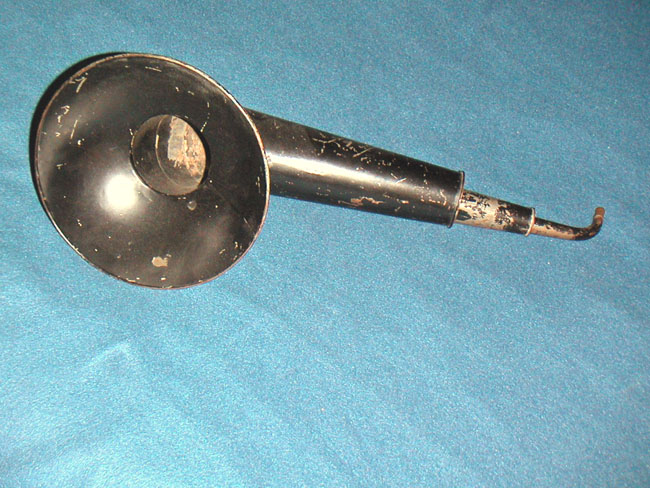
\includegraphics[width=0.5\textwidth]{trumpet}
    \caption{Trąbka słuchowa}
    \label{fig:trumpet}
\end{figure}

Pierwsze prace nad zastosowaniem sygnałów eletrycznych w~celu poprawy słyszanie przez ludzi z~ubytkiem słuchu realizował Graham Bell. Nie udało mu się osiągnąć celu, lecz na podstawie przeprowadzonych badań stworzył telefon.

W XX wieku skonstruowano pierwsze wzmacniacze elektryczne, których można było użyć do konstrukcji elektrycznych urządzeń - już aparatów słuchowych. Pierwsze maszyny były dużych rozmiarów zarówno ze względu na samo urządzenie, jak i~z~uwagi na baterię (rys. \ref{fig:siemens-old}). Postępująca miniaturyzacja pozwoliła na stworzenie urządzeń kieszonkowych w~latach czterdziestych XX wieku(rys. \ref{fig:electroear}). Kolejne generacje aparatów słuchowych coraz bardzie upodabniały się do tych znanych nam obecnie. W~latach sześćdziesiątych stworzono pierwszy aparat zauszny, obecnie najczęściej spotykany.

\begin{figure}
    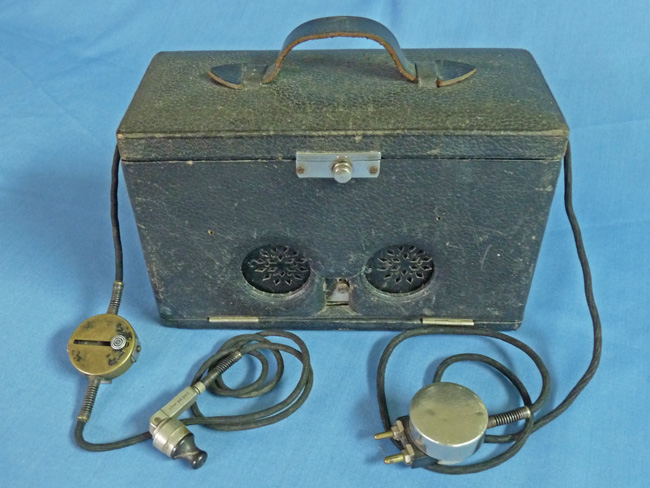
\includegraphics[width=0.5\textwidth]{siemens_old}
    \caption{Siemens/Fortiphone Model M-22 "Booster Flat" Carbon Hearing Aid}
    \label{fig:siemens-old}
\end{figure}

\begin{figure}
    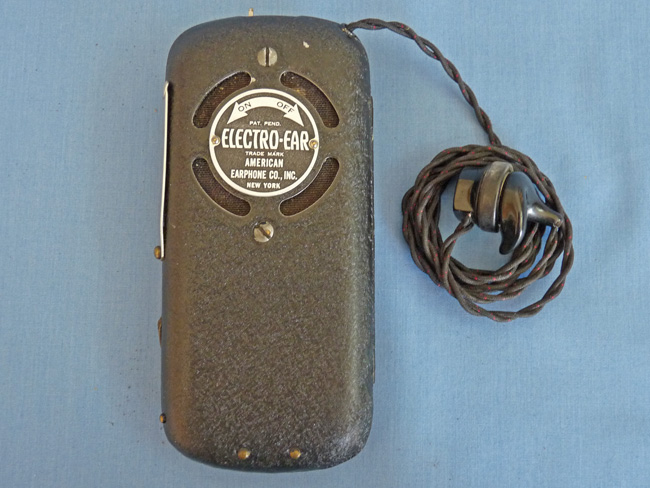
\includegraphics[width=0.5\textwidth]{electroear}
    \caption{Electro-Ear Model 5 Carbon Hearing Aid}
    \label{fig:electroear}
\end{figure}

Późniejsze aparaty stawały się coraz mniejsze oraz coraz lepiej działające. Tworzono lepsze procesory dźwięku, z~lepszymi algorytmami przetwarzania sygnału oraz z~coraz popularniejszymi dodatkowymi aplikacjami.

\section{Współczesne aparaty słuchowe}

Obecnie apraty słuchowe służą nie tylko umożliwieniu odbioru dźwięków lub poprawie słuchu. Choć jest to ich główna funkcja producenci urządzeń starają się zachęcić pacjentów dodatkowymi aplikacjami, które poprawiają działanie urządzenia (np. usuwanie sprzężeń zwrotnych), mają na celu poprawę komfortu użytkowania (np. tłumienie szumu) lub poprawiają wrażenia akustyczne(np. interpolacja dźwięku przestrzennego)

Poniżej są przedstawione najczęściej spotykane dodatki.

\subsection{Tłumienie szumu}

Prawie wszystkie modele renomowanych firm dostępne na rynku oferują tłumienie szumu i~redukcję hałasu. Ta funkcja jest dość pożądana w aparacie słuchowym z~uwagi na możliwy długi i~trudny proces dopoasowywania aparatu do pacjenta oraz uczenia się pacjenta użycia urządzenia. Dotyczy to zwłaszcza pacjentów, którzy wcześniej mieli znaczny ubytek lub całkowity brak słuchu. Odbiór dźwięku z~użyciem aparatu może odbiegać od tego, do czego pacjent był przyzwyczajony wcześniej. Dlatego korzystne jest ograniczenie ilości i głośności dochodzących dźwięku, więc taka funkcja jest bardzo przydatna.

Dodatkową funkcją jest redukcja szumu spowodowanego przez wiatr. Nie jest jednak ona oferowana w~tak szerokiej gamie modeli, jak podstawowa redukcja szumu. Nie jest to do końca uzasadnione, ponieważ szum wiatru wiejącego w~mikrofon może bardzo utrudnić słyszenie. Być może jest to tylko element marketingowy i~podstawowa funkcja tłumienia szumu pozwoli na rozumienie mowy przy wietrze. Niemniej funkcja tłumienia szumu pochodząca od wiatru jest przydatna i~powinna być obecna w~zdecydowanej większości aparatów.

\subsection{Usuwanie sprzężeń zwrotnych}

Również ta funkcja jest obecna w~większości modeli. Jest także istotna z punktu widzenia pacjenta. Podczas użytkowania aparatu słuchowego mogą powstawać sprzężenia zwrotne, które są bardzo nieprzyjemne. Dla niektórych pacjentów, zwłaszcza przy długim procesie dopasowania do apratu może być to odstraszające od używania urządzenia, mimo wszystkich jego zalet. Dlatego należy ocenić tą funkcję jako pożądaną. 

\subsection{Rożne tryby działania}

W mniejszej ilości aparatów można spotkać funkcję modyfikacji działania urządzenia w~zależności od otoczenia. Pozwala to na dokładne słyszenie w~różnych warunkach. Jest to próba odwzorowania sposobu działania naturalnego ludzkiego słuchu, które pozwala człowieku na dokładne rozumienie mowy w różnych sytuacjach. W~związku z~tym tą funkcję także można uznać za przydatną. Fakt, że jest ona obecna w mniejszej ilości aparatów pokazuje, że bez tego również mozna sprawnie funkcjonować.

\begin{figure}
    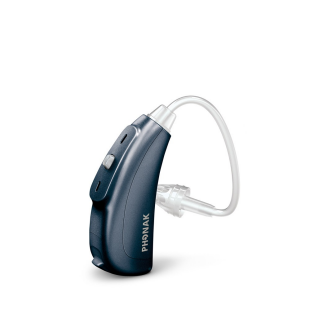
\includegraphics[width=0.5\textwidth]{phonak}
    \caption{Phonak Bolero Q}
    \label{fig:phonak}
\end{figure}

\subsection{Bezprzewodowa łączność}

Duża część aparatów pozwala na bezpośrednie podłączenie się z~innym urządzeniem, tym które nadaje dźwięk. Pozwala to na bezpośrednie przesłanie dźwięku ze źródła wprost do aparatu, dzięki czemu pomijane jest powietrze jako ośrodek rozchodzenia się dźwięku. W takiej sytuacji aparat słuchowy działa jak słuchawki. Poprawia to dźwięk dochodzący do pacjenta, który może być bez szumu z otoczenia. W~takiej sytuacji można na przykład wyciszyć odgłosy odbierane z zewnątrz. Powstaje wtedy kwestia braku kontaktu z~otoczeniem, którą należało by rozwiązać. Dla komfortu pacjenta może to mieć duże znaczenie, ponieważ dźwięk przesłany bezprzewodowo bezpośredno do urządzenia będzie lepszej jakości niż odbierany z mikrofonu aparatu słuchowego.
Ta funkcja nie jest niezbędną do użytkowania aparatu, ponieważ zawsze można przesłać dźwięk w sposób tradycyjny, z~użyciem powietrza.

\subsection{Fizyczna ochrona aparatu}

Wiele aparatów oferuję ochronę przed kurzem, wodą i~innymi zanieczyszczeniami. Część posiada także powłokę antybakteryjną. Jest to przydatna funkcja, ponieważ pozwala na korzystanie z aparatu w~deszczu lub podczas ćwiczeń (np. biegania). Dzięki temu pacjent może poprawnie słyszeć, co zwiększa jego bezpieczeństwo oraz komfort.

\subsection{Dodatkowe akcesoria}

Niektóre urządzenia oferują możliwość użycia dodatkowych akcesoriów. Są to między innymi: piloty, służące do sterowania aparatem, adaptery do różnych urządzeń pozwalające na bezprzewodową łączność, dodatkowe lub oferujące większą pojemność baterie, specjalne ładowarki do baterii, łączniki do okularów. Oferowane akcesoria nieco różnią się pomiędzy poszczególnymi firmami, ale w~działaniu są podobne. Niektóre z akcesoriów są konieczne, by skorzystać z pełnych możliwości aparatu.


\begin{figure}
    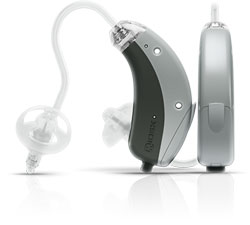
\includegraphics[width=0.5\textwidth]{widex}
    \caption{Widex SUPER}
    \label{fig:widex}
\end{figure}

\subsection{Obsługa dwóch aparatów}

W~przypadku posiadania dwóch aparatów bardziej zaawansowane modele oferują dźwięk przestrzenny. Pozwala to na słysznie, podobnie jak w~ludzkim uchu, skąd dobiega dźwięk, orientacje w~przestrzeni oraz lepsze wrażenia słuchowe. Taka funkcja jest przydatna dla osób, które mają wadę w~obydwu uszach, lecz jest zupełnie nieistnotna dla osób z~ubytkiem w~tylko jednym uchu.

\subsection{Obsługa telefonu w przypadku dwóch aparatów}

Modele droższe oferują również, w~przypadku posiadania dwóch aparatów, odpowiednie zachowanie, gdy wykryją rozmowę telefoniczną (dźwięk dobiegający tylko do jednego ucha). W~tej sytuacji urządzenia zachowują się różnie. Modele firmy Phonak przekazują dźwięk do drugiego ucha, więc pacjent odbiera rozmowę, tak jakby rozmówca był tuż obok. Aparaty firmy Bernafon wyciszają urządzenie przy drugim uchu, więc szum otoczenia staje się niesłyszalny. Podobnie jak w~przypadku dodatku powyżej ta funkcja jest dostępna dla osób posiadających dwa aparaty słuchowe, lecz niewątpliwie jest przydatna przy korzystaniu z telefonu.

\subsection{Wygląd}

Większość aparatów pozwala na personalizację wyglądu urządzenia. Zwykle dostępnych jest od kilku do kilkunastu kolorów do wyboru. Może to być istotne dla komfortu pacjenta i~akceptacji konieczności użycia aparatu. Obecnie urządzenia są małe, bardzo łatwe do ukrycia, co również może zwiększyć akceptacje pacjenta.

\subsection{Specjalne funkcje}

Aparat firmy Bernafon oferuje specjalne tryby: do słuchania muzyki na żywo oraz do oglądania filmów w~kinie. Takie tryby mają na celu poprawienie wrażeń słuchowych. W~żaden sposób nie są konieczne do poprawnego działania aparatu. 

\section{Podsumowanie}

Podsumowanie

\section{Dodatek A: }

Ewentualne dodatki


\begin{thebibliography}{123}
    \bibitem{Interton}, Strona firmy Interton.
        \url{http://www.interton-polska.pl/}
    \bibitem{Oticon}, Strona firmy Oticon
        \url{http://www.oticon.pl/}
    \bibitem{Widex}, Strona firmy Widex
        \url{http://www.widex.pl/pl-pl/}
    \bibitem{Phonak}, Strona firmy Phonak
        \url{http://www.phonakpro.com/pl/}
    \bibitem{Bernafon}, Strona firmy Bernafon
        \url{http://www.bernafon.pl/Consumers.aspx}
    \bibitem{Siemens}, Strona firmy Siemens
        \url{http://hearing.siemens.com/Global/en/products/hearing-products.html}
    \bibitem{AudioService}, Strona firmy Audio Service
        \url{http://www.audioservice.pl/}
    \bibitem{Beltone}, Strona firmy Beltone
        \url{http://www.beltone.com/index.aspx}
    \bibitem{hearingaidmuseum}, Muzeum aparatów słuchowych
        \url{http://www.hearingaidmuseum.com/gallery.htm}
\end{thebibliography}

\end{document}
